\documentclass[
    parspace,
    noindent,
    nohyp,
    %final, % hide todos
]{elteiktdk}[2023/04/10]

\usepackage{xcolor}

\usepackage{graphicx}
\usepackage{svg}
\usepackage{todonotes}
\usepackage{float}
\usepackage{pgfplots}
\usepackage{arydshln}

\newcommand{\rhpad}{\vspace{0.6\baselineskip}}

\newcommand{\thesispar}[1]{
\vspace{1em}
\hspace{0.7cm}\parbox[left][][c]{15.8cm}{\linespread{1.2}\selectfont #1}
\vspace{1em}
}

\newcommand{\longcomment}[2]{\todo[inline]{Long comment: #1}}

\usepackage[newfloat]{minted}
\AtBeginEnvironment{minted}{\singlespacing}

\title{HoloDB, egy on-the-fly virtuális relációs adattár}
\date{2023}
\author{Horváth Dávid}
\degree{Programtervező Informatikus BSc}

\supervisor{Vincellér Zoltán}
\affiliation{PhD, Mesteroktató}

\university{Eötvös Loránd Tudományegyetem}
\faculty{Informatikai Kar}
\department{Információs Rendszerek Tanszék}
\city{Budapest}
\logo{elte_cimer_szines}


\addbibresource{references.bib}

\begin{document}

\documentlang{hungarian}

\listoftodos
\cleardoublepage

\makecover
\cleardoublepage

\maketitle

\tableofcontents
\cleardoublepage


\begin{abstract}
A szofisztikált tesztelés és a gyors prototípusgyártás
a modern szoftvertechnológia két elengedhetetlen alapköve.
Mégis, ezek egyik fő függőségének, a teszt- illetve demóadatoknak
a rendelkezésre állása manapság is komoly kihívást jelent.
Általában két megközelítési móddal találkozunk:
vagy az adatok on-the-fly generálával, mely ugyan kisköltségű,
de teljesen inkonzisztens az egyes üzenetváltások között;
vagy valamilyen tesztadatbázis odahelyezésével,
mely nem csak hogy hordozza a tényleges adatbázis minden költségigényét,
de jellemzően számos további nehézséggel bővíti, például adatgenerálással vagy anonimizálással.
Dolgozatomban egy olyan megoldás alapjait mutatom be,
mely további előnyök mellett ötvözi az előbbi kettő erősségeit,
míg kikerüli azok fő hátrányait.
Az előterjesztett megoldás egy akár közel zéró erőforrásigényű virtuális relációs adattár,
melynek szerkezete és adattartalma konfigurációs fájlon keresztül rugalmasan paraméterezhető,
és a lekérdezéseket on-the-fly hajtja végre konzisztensen
(legyen az SQL, NoSQL, GraphQL vagy egyéb),
és performanciája legalábbis összemérhető a valódi adatbázisokéval.
Ez a performancia akkor érhető el, ha a virtuális adatokhoz virtuális indexek is tartoznak,
aminek implementációbeli magját többek között a rendezett értékkészletek,
a diszkrét monoton függvények
illetve a kriptográfiában is használatos megfordítható permutációk adják.
\end{abstract}

\chapter{Áttekintés}

\section{Egy mindennapi probléma}

A szoftverfejlesztési és -release-elési folyamatok lényeges előfeltevése,
hogy az alkalmazás mint absztrakt entitás snapshot jellegű,
azaz a mindenkori forráskód \textit{aktuális állapotának} determinisztikus derivátuma,
nem függ annak történetiségétől.
Ezt az átlátható képet bolygatja meg a szoftverhez tartozó produkciós adatbázis,
mely önálló életet él, a felhasználói világgal való interakcióban folyamatosan változik;
szerkezete, szemantikája azonban szorosan az alkalmazás mindenkori állapotához kötődik.

Ez a kettős természet legalább két nagy problémakört eredményez.
Az egyik a verziókezelést érinti:
a produkciós adatbázist csak differencia-szkriptek végrehajtásával tudjuk módosítani,
ami jellemzően egy másodlagos verziókezelést eredményez a forráskód verziókezelésén belül
(ilyen megoldás például a Flyway vagy a Liquibase),
és sorozatos összefésülési problémákhoz vezet, ha az adatok szerkezete vagy szemantikája gyakran változik.
A jelen dolgozatban nem foglalkozom ennek a kérdésnek a részleteivel,
de az utolsó felyezetben vázolom majd egy lehetséges megoldás körvonalait,
ami szervesen következik majd az azt előzőekből.

A másik problémakör azzal kapcsolatos, hogy ugyan az ``életnek kitett'' produkciós adatbázist
kénytelenek vagyunk minden erőforrásigényével életben tartni valamint minden release-zel migrálni,
ám az absztrakt értelemben vett mindenkori adatbázisra számos egyéb helyen is szükségünk van,
ahol ezek a folyamatos költségek igencsak nemkívánatosak.
Ilyenek jellemzően:

\begin{itemize}
    \item adatfüggő stubok és mockok
    \item integrációs és egyéb tesztek
    \item gyors prototípusgyártás, kísérletezés, draft adatbázisok
    \item rövid demonstrációk, prezentációk
\end{itemize}

Ezeken kívül, ha egy csak-olvasható adattartalmat akarunk nagy adatforgalomnak kitenni,
fölmerülhet az adattartalom replikálása, és load-balanceren keresztüli elérhetővé tétele,
ekkor azonban minden újabb példány jelentősen növeli a tárhelyfoglalást.

Nem is mindig áll rendelkezésre egy produkciós adatbázis,
amikor éppen jól jönne belőle egy másolat.
De amikor rendelkezésre is áll, tartalma általában érzékeny adatokkal van tele,
melyeket nem is használhatunk fel csak úgy (anonimizálás nélkül) egyéb célokra.

Más területeken is találkozhatunk a fentiekhez hasonló kívánalmakkal.
Például az adatbázisok oktatásában is jellemző, hogy minden egyes hallgató
számára elérhető saját izolált adatbázis adatbázist bocsátanak rendelkezésre,
bár mindegyik ilyen adatbázis szükségszerűen ugyanazzal a szerkezettel és adatokkal bír.

Fogalmazzuk meg tehát a problémát, mintegy tézisként:

\thesispar{
    \textbf{Alapmegállapítás:} Igen gyakran ütközünk abba a helyzetbe, hogy adott struktúrájú és szemantikájú
    viszonylag rövid életű adatbázist kell biztosítani,
    a produkciós adatokra vonatkozó speciális követelmények nélkül.
}

A fejezet további részében röviden végigveszem, hogy általában hogyan szokás a hasonló problémákat megkerülni,
majd rátérek a az általam javasolt megoldás nagy vonalakban történő ismertetésére.
Ezt követően pedig táblázatba foglalva összevetem mindezek előnyeit és hátrányait.
Végül az utolsó szakaszban megkísérlem megtalálni az okát,
miért hiányzik 

\section{Körkép}

\subsection{Kérések mockolása on-the-fly}

Főként webes API-k által szolgáltatott adathalmazok mockolásakor találkozunk olyan megoldással,
mely a lekérés (és persze az előre beállított szabályok)
alapján generálja a válaszként visszaadandó adatstruktúrát
(például egy rekordot vagy dokumentumot JSON formátumban).
Az adatok véletlenszerűen kerülnek kitöltésre a lekérés szerkezete alapján megállapított schema keretébe.

A módszer SQL-lekérdezések közvetlen mockolásához is adaptálható,
a lekérdezés (és ha ismert, akkor a schema) alapján meg kell állapítani
a visszaadandó eredménytábla szerkezetét, adattípusait,
az egy-egy oszlopba kerülő adatok jellegét,
majd random jelleggel elő kell állítani bizonyos számű, ezeknek a követelményeknek megfelelő eredményrekordot.

Ez a megoldás természetesen nem fog konzisztens eredményt adni több lekérés esetén,
így csak olyan esetben használható, ahol a lekérések nem épülnek egymásra.
Cserébe erőforrásigénye csekély, nincs szükség az adatok tényleges tárolására.

\subsection{Seed alapú virtuális világok}

Egyszerűbb szimulációkban és játékokban már igen régen generálnak kisebb világokat,
pályákat procedurálisan valamilyen pszeudo-random algoritmus segítségével.
A módszer továbbfejleszthető óriás világokra is.
Ekkor a világteret (sorosan vagy hierarchikusan) szeletekre osztjuk, és biztosítunk egy függvényt,
mely minden szelethez rendel egy saját seed értéket.
Legegyszerűbb esetben a seed az adott szelet sorszámából generált hash.
Amikor szükségünk van valamely szelet tartalmára, az adott szabályrendszer szerint
a szelet seedjéből kiindulva on-demand legeneráljuk az adott szelet tartalmát.
A sűrűn benépesített világok szomszédos szeleteinek összeillesztése néha nem triviális.
Felületek generálása esetén gyakran használnak valamilyen eleve interpolált eljárást, például Perlin-zajt,
így biztosítva a közeli helyeken a közeli értékeket.

Egy közismert korai példa seed alapú módszert alkalmazó szoftverre
az Elite nevű 1984-ben kiadott űrhajós videójáték.
A játékban meglátogatható bolygók kapnak egy-egy seedet, mely már teljesen meghatározza a felépítésüket,
így elég a bolygó meglátogatásakor legenerálni a tartalmát.
A módszert utána számtalan óriástérképes játék vette át.

Ha elvonatkoztatunk a játékoktól és szimulációktól,
ez a generálási módszer közel tetszőleges jellegű virtuális adathalmaz böngészését képes biztosítani.
De azonnal szembeötlik a legfőbb hátrány is: a virtuális világ-adathalmaz nem kereshető.
Nem tudjuk például hatékonyan lekérdezni, mely világszeletekben lelhető föl egy adott típusú objektum.

\subsection{Relációs adatok generálása}

Amikor adatokat generálunk egy relációs modellbe, azt legegyszerűbb megközelítésben fölfoghatjuk úgy is,
mint az előbb bemutatott virtuális világ materializációját egy relációs adatbázisszerveren.
Milyen előnyöket nyerünk ezzel? Lássunk néhányat:

\begin{itemize}
    \item utófeldolgozás: utólag holisztikus módosításokat eszközölhetünk az adathalmazon
    \item egynemű módosíthatóság: minden eleve tárolva van, nem kell külön kezelni a változásokat
    \item kereshetőség: az adatbáziskezelő biztosítja az indexeket
\end{itemize}

A fő hátrány egyértelmű: a nagy tárhelyigény.
Vegyük észre, hogy még a kereshetőség is az indexek által foglalt további tárhely által valósul meg
(az adatok eleve nagy tárhelyfoglalása mellett tűnhet esetleg elhanyagolhatónak).
Ha pedig nem materializált adatok mellé gyártunk indexeket,
akkor ki kell dolgoznunk valamilyen módszert a módosulások detektálására, ami általában nem triviális.

Egyes generátorok a schema és az adatok jellegének deklaratív leírását is támogatják. Ez a leírás tárolható egy konfigurációs fájlban, ami verziókezelhető, dokumentálható, könnyen szerkeszthető.

\subsection{Relációs adatok anonimizálása}

Ha már rendelkezésre áll egy éles adatbázis, kézenfekvőnek látszik,
hogy ennek replikáit használjuk a teszt- vagy mockadatbázis kiindulópontjaként.
Így rögtön egy valószerű adatokhalmazzal indulunk, az érzékeny adatok miatt azonban anonimizálásra van szükség. Tehát a generáláshoz szükséges számítási igényt összességében
felcseréljük a másolás és anonimizáció költségeivel.

Úgy tűnik, gyakran anonimizálással együtt is egyszerűbb valós adatokból kiindulni,
mint egy komplett generálási folyamatot kiépíteni.
Egy köztes megoldás lehet a schema és az adatok nagyjábóli jellegének letapogatása,
és az ez alapján történő újragenerálás.

Azonban a bevezetőben felsorolt szituációk egy részében nem áll rendelkezésre egy létező produkciós adatbázis.
Emiatt egy általános megoldás aligha épülhet aninimizálásos módszerre.

\subsection{Nagy teljesítményű megoldások}

Számos nagyteljesítményű megoldás érhető el a piacon, amellyel szintetikus adatok generálhatók. A MOSTLY AI megoldása az akkurátus adatokra helyezi a hangsúlyt. Az adatok statisztikai jellemzői és mintázatának lényeges elemei jól illeszkednek a valós adatoknál látható mintázatokra.

Egyes platformok általános megoldást nyújtanak az adatgenerálásra, anonimizációra és CI/CD-integrációra.
Ilyen például a Tonic, a GenRocket és a Delphix.

Ezek a rendszerek erősen optimalizálják és párhuzamosítják a tesztadatok előállításának egyes lépéseit,
így a fapados megoldásokhoz képest költséghatékonyak.
Csodát viszont nem lehet várni: a számításigény aszimptotikusan,
a tárhelyigény pedig teljes egészében ugyanaz marad.

\section{A betöltésre váró hézag}

Az előzőekben tárgyalt megközelítések mindegyikének megvoltak a maga sajátos előnyei ás hátrányai.
Fölmerül a kérdés: létezhet-e olyan megoldás, amely egyesíti az előnyöket és kikerüli a fő hátrányokat;
vagy pedig ez eleve lehetetlen?

Először szedjük össze tételesen, milyen követelményeket várnánk el
egy (egyelőre hipotetikus) ideális készterméktől:

\begin{itemize}
    \item támogatja a relációs adatmodellt, mint legáltalánosabbat
    \item determinisztikus, konzisztens, és egy root seed módosításával újrakeverhető
    \item azonnal elindul, nincs számottevő preparálási folyamat
    \item az adatokat csak elérésükkor, on-the-fly számítja
    \item indexeket szolgáltat, ahol az egyébként is elvárható lenne
    \item könnyen és rugalmasan konfigurálható, fájlon keresztül is
    \item óriás adatmennyiséget is képes szimulálni
    \item skálázható, finomhangolható
    \item egyedi működéssel könnyen bővíthető
    \item opcionálisan írható
\end{itemize}

Az utolsó, írhatósági követelménynél föltehetjük, hogy az ilyen adatbázis viszonylag rövid életű,
tehát nincs szükség sem nagy mennyiségű módosítás megjegyzésére, sem azok hosszú távú perzisztálására.
Így az egynemű módosíthatóság fentebb említett előnyét nyugodtan elvethetjük.
Ha egyszer a módosítási réteg megfelelően és univerzálisan implementálva van,
az egyes felhasználásoknál már nincs ezzel kapcsolatos teendő.

Belátható, hogy a fenti elvárások egyszerre teljesíthetők.
Az alábbi szekcióban röviden vázolom, milyen ötletek és tervezési elvek alakították ki a megoldásom.
Az implementáció részleteit a következő fejezetben fogom bemutatni.

\section{Egy újfajta megoldás körvonalai}

A következőkben leírt szoftvernek már létezik egy prototípusa HoloDB[hiv!] néven.
Mivel ez Java nyelven íródott, a továbbiakban implicite felteszem, hogy Java környezetben vagyunk.

Megoldásom mindenekelőtt egy relációs adatbázist leíró API-t fog definiálni illetve megvalósítani.
Aligha érdemes más megközelítést választani,
hiszen a relációs adatmodell nem csak tradicionálisan megkerülhetetlen
és máig a legnépszerűbb adattárolási módszer[hiv!],
de egyúttal közös nevezőként szolgál bármely más modellhez.
Egy relációs struktúrával gyakorlatilag bármilyen interpretált adathalmazt le tudunk írni,
mivel a relációs séma általános normalizációs segédeszköz.

Hamar arra a megállapításra jutottam, hogy a releváns értelemben legalapvetőbb objektum
az \textit{oszlop}.
Az oszlop alatt azonos típusú adatokat találunk,
és az első feladat mindig ezen adatok értékkészletének megadása.
Általában egy index is egy (esetleg néhány) konkrét oszlophoz köthető.

Természetesen hamar ki kell lépnünk a teljes oszlop-orientáltságból.
Lehetnek összefüggések például egy táblán belül oszlopok között,
de ezt még mindig egyszerűbb az oszlopos megközelítés megfelelő kiterjesztésével elérni,
mintsem áttérni valamiféle rekordonkénti generálásra.
Az oszlopok alatti mezők jó jelöltek arra, hogy ``világszeletek'' legyenek,
míg egész rekordok nem.

Illetve lehetnek megkötések táblák között is.
Ezek kezelése is könnyen elvégezhető az oszlopos alapvetésre építve.
Az egészszámos idegen kulcsoknál például csak annyit kell biztosítani,
hogy a hivatkozó oszlop értékkészlete a hivatkozottnak a tartalma legyen.

A legtöbb oszlop értékkészlete jól behatárolható.
A tényleges értékek egy efölötti multihalmazt alkotnak,
néha ehhez valamilyen statisztikai megkötés is tartozik ($NULL$-ok száma, értékgyakoriság stb.).
Továbbá a multihalmaz valamilyen konkrét sorrendben helyezkedik el az oszlop alatt.
Itt jegyzem meg, hogy a tábla rekordjait sorrendezettnek fogom tekinteni:
azonos táblabeli valamely két oszlop értéklistájából kiválasztott egy-egy mező
azonos rekordhoz tartozik pontosan akkor, ha a sorrendbeli pozíciójuk (sorindexük) megegyezik.

Vegyük észre, hogy két független problémával szembesülünk:

\begin{enumerate}
    \item az oszlopértékek multihalmazának előállítása
    \item az értékek összekeverése
\end{enumerate}

Ezeket úgy kell megvalósítani, hogy a végső értéklista adott pozíciójú eleme is gyorsan lekérhető legyen,
valamint egy adott érték vagy értéksáv előfordulási pozíciói is
(utóbbi esetben lehetőleg rendezetten).
Ha feltesszük, hogy a multihalmaz úgy van ábrázolva,
hogy a hatékony értéklekérés és keresés-rendezés elvárása teljesül,
akkor már csak egy (a tábla hosszára értelmezett) invertálható permutációra van szükség,
hogy az adatokat visszakereshetően szét is szórjuk.
(Lentebb látni fogjuk, milyen módszerrel tudjuk a multihalmaz egy (eleve rendezett) reprezentációját képezni,
amivel az elvárások teljesíthetők.)

Gyorsan számítható invertálható permutációk például modulo szorzásból kiindulva valósíthatók meg.
Költségesebb, de erősen véletlenszerű összevisszaságot bitzosító invertálható permutációkat
különféle kriptográfiai módszerekkel állítok elő.
Többéle algoritmuscsalád kipróbálása után (pl. Format Preserving Encryption) végül
a hosszigazított Feistel-hálózat alkalmazása bizonyult a legkezelhetőbbnek.

A kétfázisú értékiosztásnak ezzel az ötletével
egy egyszerűbb adatbázis szimulációjának kívánalmait már tulajdonképpen le is fedtük,
de néhány további hasznos értékkiosztási módszert is be fogok majd mutatni.

Az értékkészlet esetenként óriási lehet,
gondoljunk például a reguláris kifejezés alapján kitöltött oszlop lehetséges értékeinek számára.
Az on-the-fly értékszámítás során gyakran fordulnak elő átmeneti óriás számok,
ám nehezen jósolható, hogy pontosan mikor.
Emellett az adatbázis méretére vonatkozóan sem akartam megkötéseket tenni.
Nem lett volna célszerű explicit ellenőrzések tömegét beépíteni
a problémás számítások, potenciális túlcsordulások földerítésére.
Az egész számokat egységesen szerettem volna kezelni, függetlenül azok méretétől,
így a \texttt{BigInteger} típus használata eleve kiesett,
mivel az kisebb számokra a \texttt{long} típushoz képest rendkívül rossz performanciájú.

Az értékkiosztási trükkökkel egy statikus adatbázist írunk le,
ami értelemszerűen önmagában csak-olvashatóan érhető el.
Látni fogjuk, hogy lehet egy csak-olvasható tábla fölé olyan dekorátort helyezni,
mely a változások megfelelő adatstruktúrában történő számontartásával
az írhatóság illúzióját kelti.

Ha a relációs adatmodell objektumait (oszlopok, táblák, indexek stb.) sikeresen implementáltuk,
a relációs műveletek (és így az SQL nyelv) megvalósítása már a szokásos módon történhet.
Ma már elérhető néhány nyílt forrású jól felépített SQL query planner framework,
ami lehetővé teszi egy teljeskörű SQL-szerver kiépítését.
Ilyen például az általam használt Apache Calcite
(Ugyanakkor egy saját SQL-futtatót is implementáltam,
mely a nyelv limitált verzióját támogatja, de néhány esetben gyorsabban fut).

A virtuális adatbázis felépítése a felhasználó számára legegyszerűbben
egy konfigurációs fájl segítségével történik,
melyben megadja az adatbázis-séma egyes elemeit, megkötéseit.
Az oszlopok tartalmának keverési módja és értékkészlete kényelmesen állítható,
például előre adott értéklistákkal, reguláris kifejezéssel,
vagy a felhasználó által implementált Java-osztállyal.
A virtuális adatbázis dockerben való indításához vagy beágyazott használatához
lényegileg elég egy ilyen konfigurációs fájl.

\section{Az új megközelítés előnyei}

Ha a virtuális adatbázis legegyszerűbb használati módját tekintjük,
a felhasználói élményben három lényeges fázist különíthetünk el.
A figyelem először a konfigurációs fájlra irányul:
egyetlen átlátható, deklaratív, verziókezelhető adatfájlban minden megadható, amire szükség van.
Majd az adatbázis létrejötte és a szerver elindulásakor feltűnik,
hogy teljesen hiányzik a szokásos másolási, generálási, anonimizálási, inicializálási vagy egyéb folyamat,
a szerver töredékmásodperc alatt válaszképesen elindul.
Végül futási időben az látszik, hogy a szerver rendkívül kis memóriaigénnyel fut
(ez csak a módosításokkal arányban változik valamelyest),
ugyanakkor a lekérdezések futási ideje sem marad el nagyságrendekkel a tényleges adatbázisétól.

Az integrált konfigurációs fájl előnye még,
hogy létező adatbázispéldányokon tanított mesterséges intelligencia segítségével is generálható.
Az MI-alapú konfigurációmenedzsent egyre szélesebb körben alkalmazott módszer,
megtaláljuk a SAT-solverektől[hiv!] a felhőarchitektúrákig[hiv!],
nem látszik elvi akadálya az adatbázisra vonatkozó konfigurációban való alkalmazásnak.

De ilyen vaskos módszerek nélkül, egyszerűbb heurisztikákkal is lehetséges
egy létező adatbázis jó közelítéssel történő letapogatása.
Hasonlóan, a virtuális adatbázis könnyen renderelhető egy valós adatbázisba.

Arra is lehetőség van, hogy a konfiguráció a JPA entitások
(és opcionálisan az azokra helyezett specializált annotációk)
alapján generálódjon, például adatbázisos tesztek futtatásához.

A könnyűsúlyú jelleg olyan új távlatokat nyit, amelyek korábban föl sem merülhettek.
Például most már nincs akadálya, hogy bármely füstteszt adatbázis-eléréssel fusson.
A CI/CD pipeline-okban adathalmazok kívülről való betöltése nélkül is lehet rövid feladatokat futtatni.

Azt hiszem, jogosan merül föl a kérdés, hogy miért nem született és terjedt el még hasonló termék.
Ennek fő okait az alábbiakban látom:

\begin{itemize}
    \item \textbf{kontraintuitivitás}: előzetes feltevésemmel szemben úgy tűnik,
          nem olyan egyszerű átlátni a koncepciót, és megérteni hogy ``hol is vannak az adatok''
    \item \textbf{megfelelő SQL plannerek eddigi hiánya}: az Apache Calcite például
          csak az utóbbi néhány évben vált népszerűvé, és inkább elsősorban adatintegrátorként
    \item \textbf{bejáratott alternatívák}: az adatnélküli mockolás lehetősége,
          a NoSQL adatbázisok elterjedése, a felhőmegoldások fejlődése stb.
          szenderképző kerülőmegoldásokként elfedték a problémát
    \item \textbf{érdekhiány}: a releváns területen működő nagyobb vendorok elsősorban
          erőforrásokat adnak bérbe, és az általuk fejlesztett architektúrák (történetileg érthetően)
          elsősorban az ezeken futó tényleges adatbázisok kezelését kell megoldják;
          nincs tehát nyomás jelentősen más típusú termékkel való kísérletezésre
\end{itemize}

A következő táblázat összehasonlítja megközelítéseim és a létező megoldások fő jellemzőit:

\begin{table}[H]
\settowidth\rotheadsize{mmmmmmmmmmmmmm}
\begin{center}
\begin{tabular}{ |c|c c c c:c c| }
  \hline
  \begin{tabular}{ l l } ~ \\ ~ \\ XXXX / \\ YYYY\end{tabular} &
    \rothead{Adatgenerálás \\ \textit{külső} adatbázissal} &
    \rothead{Adatgenerálás \\ \textit{beágyazott} adatbázissal} &
    \rothead{Produkciós adatbázis \\ másolatának használata} &
    \rothead{Anonimizálás a \\ produkciós adatbázisból} &
    \rothead{A jelen megoldás \\ \textit{konténerben} futtatva}&
    \rothead{A jelen megoldás \\ \textit{beágyazva}} \\
  \hline
  \parbox{2cm}{\rhpad Item 1 \rhpad} &
    ((AAA)) &
    ((BBB)) &
    ((CCC)) &
    ((DDD)) &
    ((EEE)) &
    ((FFF)) \\
  \parbox{2cm}{\rhpad Item 2 \rhpad} &
    ((AAA)) &
    ((BBB)) &
    ((CCC)) &
    ((DDD)) &
    ((EEE)) &
    ((FFF)) \\
  \hline
\end{tabular}
\end{center}
\end{table}

\todo[inline]{még az elején is valami ábra vagy tábla}
















\chapter{A virtuális adattár}









\section{XXX}

\todo[inline,color=red]{XXX}

\todo[inline,color=red]{generálás adatfából (ua. mint a regex), valós címek stb.}

Előző változat bevezető fejezetei:

\begin{itemize}
    \item Végtelenített virtuális világok
    \item A fakerek limitációi
    \item Néhány visszatérő probléma közös nevezője
    \item A fakerek limitációi
    \item Virtuális mockolás: hézag jelei új termék számára?
    \item \dots
    \item Felépítés
    \item Konfiguráció
\end{itemize}

Egyéb:

\begin{itemize}
    \item determinisztikus, de a seed-del variálható//összekeverhető
    \item Relational data as a serverless function
    \item SQL, NoSQL, GraphQL, REST etc.
    \item miniconnect, minibase, REPL
    \item a konfiguráció előfeldolgozható (pl. yaml + go template, mint a helmnél)
    \item valós adatbázis feltöltése innen
    \item konfiguráció generálása
    \begin{itemize}
        \item valós adatbázis egyszerű feldolgozásával
        \item valós adatbázis intelligens feldolgozásával (pl. evolúciós algoritmussal)
        \item valós adathalmazokon tanított AI által
    \end{itemize}
\end{itemize}

[az előzőek alapján a kétdés végülis: tudunk-e úgy virtuális adatvilágot szolgáltatni, hogy azokhoz indexek is tartozzanak? (--> storage API)]
[világos, hogy a run-time performanciából vesztünk (de nem vészesen!), a lényeg, hogy más lényeges hátrány nem nagyon van]
[teljesítményteszt kell egyszerűbb querykkel, illetve bonyolulttal is calcite-tal]
[a rendezés vs. join problémát javítani]
[ahol nem kell kereshetőnek lenni, ott tulajdonképpen a normál seedes szeletenkénti világgenerálás játszik]
[konfigot kiegészíteni még egyedi működés támogatásával]
[calcite minimális támogatása]





\section{A \texttt{LargeInteger} típus}

Az adatok on-the-fly számításakor a szűk keresztmetszet
a tárolás és elérés problémáiról a kalkulációkra helyeződik át.
Nyilvánvaló tehát, hogy az egész koncepció sikere azon áll vagy bukik,
hogy milyen gyorsan tudjuk számítani az eredményt.

A legtöbb oszloptípusnál rendezett értékkészletbeli pozíciókat mappelünk össze sorindexekkel.
Az értékkészlet óriási is lehet,
illetve számos további részeredmény esetében merül föl az óriás számok problémája.
Ezért szükségesnek mutatkozott egy olyan egész típus megalkotása,
mely kis és óriás számokra egyaránt működik,
és kis számok esetében nagyon hatékony (ellentétben a beépített \texttt{BigInteger} típussal).

Az ecélból készített (egyébként teljesen általános) \texttt{LargeInteger} típus
valójában egy interfész két privát implementációval:
az \texttt{ImplSmall} a \texttt{Long.MIN\_VALUE}-tól a \texttt{Long.MAX\_VALUE}-ig
terjedő intervallumra (kis számok),
az \texttt{ImplBig} pedig az ezen kívül eső értékekre (nagy számok) optimalizálva.

Az \texttt{ImplSmall} egy primitív \texttt{long} értéket tárol.
Az egyes műveletei esetében egy olcsó ellenőrzéssel mindig megállapítja,
hogy biztos-e, hogy nem lesz túlcsordulás.
Ha ez biztos, akkor a műveletet primitív műveletként végzi el.
Ha nem biztos
(vagy azért, mert az ellenőrzés nem zárta ki a túlcsordulást,
vagy mert nagy számot kapott operandusként),
akkor a \texttt{BigInteger} segítségével hajtja végre a műveletet;
ha az eredmény mégis kis szám, akkor \texttt{ImplSmall} példányként adja vissza.

Az \texttt{ImplBig} mindig a \texttt{BigInteger}-en keresztül végzi a műveleteket.
Hasonlóan a másik implementációhoz, szintén ellenőrzi, hogy az eredmény kis szám-e,
Általában, egy \texttt{LargeInteger} szám akkor és csak akkor csomagolódik \texttt{ImplBig}-ként,
ha kívül esik a \texttt{long} értékkészletén.

A \texttt{LargeInteger} a \texttt{BigInteger} összes metódusát replikálja,
illetve számos további kényelmi metódust ad hozzá.
A zérusközeli értékek gyorsítótárazva vannak a hatékonyság további növelése érdekében.

A Scala standard könyvtárának \texttt{BigInt} típusa szitén a \texttt{long} és \texttt{BigInteger}
aritmetika váltogatásával oldja meg,
hogy az óriás számok támogatása mellett kis számokon viszonylag gyorsan fusson.
A két megoldás performanciában hasonló,
néhány jelen esetben releváns esetben (kisebb számok, sokféle művelet)
a \texttt{LargeInteger} valamivel gyorsabb.

\begin{figure}[H]
    \centering
    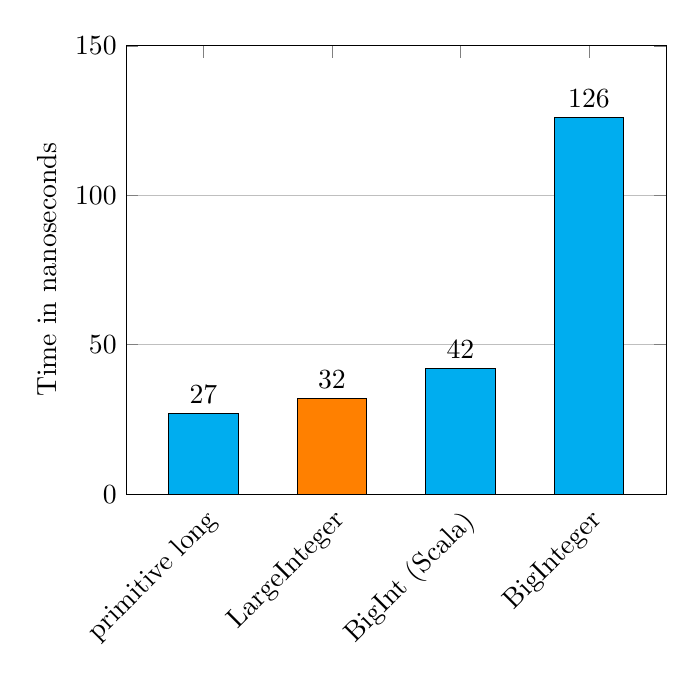
\begin{tikzpicture}
        \begin{axis}[
                symbolic x coords={primitive long,,LargeInteger,,BigInt (Scala),,BigInteger},
                xticklabel style={rotate=45,anchor=north east},
                xtick={primitive long,LargeInteger,BigInt (Scala),BigInteger},
                ylabel=Time in nanoseconds,
                ymajorgrids,
                ymin=0,
                ymax=150,
                bar width=25pt,
                enlarge x limits=0.2,
                nodes near coords,
                nodes near coords align={vertical},
            ]
            \addplot[ybar,fill=cyan] coordinates { (primitive long,27)};
            \addplot[ybar,fill=orange] coordinates { (LargeInteger,32) };
            \addplot[ybar,fill=cyan] coordinates { (BigInt (Scala),42) };
            \addplot[ybar,fill=cyan] coordinates { (BigInteger,126) };
        \end{axis}
    \end{tikzpicture}
    \caption{
        A \texttt{LargeInteger} teljesítményének összehasonlítása
        egy kis számokon végzett összetett számítás átlagos futási ideje alapján
    }
\end{figure}

\todo[inline]{további LargeInteger-alternatívák teljesítményének vizsgálata}

\section{A TreeRandom és kapcsolódó API-k}

\todo[inline]{section: A TreeRandom és kapcsolódó API-k}

\section{A storage API}

\todo[inline]{section: A storage API}

\longcomment{Storage API ötletelés}{
schemák, táblák és oszlopok
indexek
   normál
   rendezetlen (optimalizálás-egyszerűsítés, kezelhető normál indexek halmazaként is)
   full-text
   spatial???
}

\section{A csak-olvasható alapréteg}

Bármilyen imlementáció legyen is mögötte, a storage API egy relációs adatbázist ír le.
Tehát ahhoz, hogy a virtuális adatok funkcionálisan egy valódi (csak-olvasható) relációs adathalmaz képét adják,
nem kell más, mint hogy konzisztens módon elérhetők legyenek a storage API-n keresztül.
A konzisztencia ez esetben két dolgot jelent:

\begin{enumerate}
  \item Felépíthető egy olyan tényleges immutábilis relációs adatbázis ($M$),
        hogy minden lehetséges relációs lekérdezés esetében, amely a közös schemára ($S$) értelmes,
        a virtuális és a tényleges adatbázis esetében visszaadott eredménytábla megegyezik.
  \item Az $S$ schema teljesíti a virtuális adatbázis felhasználói konfigurációját ($C$),
        valamint az $M$-ben szereplő adatok tulajdonságai illeszkednek a $C$-ben leírt megkötésekre.
\end{enumerate}

A virtuális adatokhoz a legalsó szinten a storage API megfelelő hívásaival férünk hozzá.
Ezek a speciális hívások szűk keresztmetszetet képeznek,
hiszen ezek szimulálják például a közvetlen adatelérést is.
Ha ezen hívások performanciája nagyságrendileg (de legalább aszimptotikusan) összemérhető a tényleges adatbázisokéval,
akkor az erre épülő lekérdezésfuttató és egyéb rétegek már
a tényleges adatbázisoknál megszokott módon és nagyságrendi teljesítménnyel tudnak működni.

A lekérdező műveletek esetében két különösen fontos hozzáférési módot kell kiemelni:

\begin{enumerate}
  \item rekordok véletlen elérése (random access)
  \item adott érték előfordulásainak keresése egy oszlopban (reverse index)
\end{enumerate}

Ha e két hozzáférési mód hatékony, akkor már a lekérdezések jelentős részénél
elérhető a tényleges adatbázisokéval összemérhető performancia.

A storage API-ban úgy definiáltuk a megfelelő interfészt,
hogy a keresésen kívül még néhány további funkciót is támogatnia kelljen,
például a rendezést és a $NULL$ értékek kezelését.
A következőkben leírt értékkiosztási módszerek többéségénél természetes módon következik,
hogy ezeket a további elvárásokat is teljesítik.
Az e szempontból problémás esetekre külön ki fogok térni.

\todo[inline]{További megjegyzések a csak-olvasható alapréteghez}

\section{Megoldások a hatékony értékkiosztásra}

Virtuális adatok alatt elsősorban az egy-egy oszlop alá besorakozó,
közös típussal rendelkező mezőértékeket értem.
Úgy is fogalmazhatunk, hogy az adatokat alapvetően oszlop-orientáltan fogjuk előállítani.
Minden oszlophoz tartozik majd egy virtuális adatlista,
melynek hossza egyenlő az adott oszlopot tartalmazó tábla hosszával
(opcionálisan szerepelhetnek benne $NULL$ értékek),
a többi érték típusának pedig kompatibilisnak kell lennie az oszlophoz megadott típussal.

Bár ez a megközelítás oszloponként független adatlistákra van szabva,
valójában más jellegű értékkiosztási módszer is lehet mögötte,
amennyiben az egy-egy oszlophoz tartozó listanézetek biztosítottak.
Majd a több oszlopot érintő megkötések esetében ez lesz a helyzet.
De lássuk először az egyoszlopos értékkiosztások lehetséges módszereit.

\subsection{Indexelt egyoszlopos értékkiosztások}

\subsubsection{Előzetes megfontolások}

E következőkben olyan értékkiosztási módszereket veszek végig,
amelyek lehetőleg biztosítják az alábbiakat:

\begin{enumerate}
  \item hatékony elérés (random access)
  \item pozíciótól függő érték (seed + sorindex)
  \item hatékony kereshetőség valamilyen formában
  \item hatékony rendezés
\end{enumerate}

Az egyes esetekben megvizsgálom majd, hogyan teljesíthetők ezek az elvárások.

\subsubsection{$NULL$ értékek kezelése}

Általánosan, bármely értékkiosztási módszerhez könnyen hozzáilleszthető a $NULL$ értékek támogatása.
Mindössze az szükséges, hogy az értékkiosztást a tábla méreténél kisebb intervallumra végezzük,
a maradék helyeket pedig $NULL$-nak tekintjük.
Ezen felül opcionálisan egy permutáció beiktatásával az értékeket elkeverhetjük,
ami által a $NULL$ értékek is szétszórtan szerepelnek majd.

Nem szükséges ez a plusz kompozíció,
ha a fentiek magába az eredeti értékkiosztásba is könnyen beépíthetők.
Például a kétfázisú értékkiosztásokba egyszerűen felvehető a $NULL$ mint érték.

Akár beépítetten, akár plusz kompozícióval van megvalósítva a $NULL$ értékek kezelése,
természetesen figyelni kell a speciális kezelésre a keresés-rendezés során.

A fentiek fényében az egyes értékkiosztások tárgyalásánál a $NULL$ értékek kezelésével nem foglalkozom.

\subsubsection{Egyszerű értékkiosztások}

Tényleges adatbázisokban némely esetben meglehetősen következetes módon
szerepelnek az értékek az oszlop értéklistájában.
Természetesen az ilyen esetek szimulálása a legegyszerűbb.

Triviális eset, ha egy oszlop mezői egy közös konstans értéket tartalmaznak.

Továbbá, ha olyan adathalmazt szimulálunk, melyre megengedhető a feltevés,
hogy sem törlés, sem releváns értelemben problémás felülírás nem történt még,
úgy egyes oszlopok szekvenciális alapon generálhatók.
Az ilyen esetekben az $n$-edik érték lekérése
egy egyszerű lineáris függvénnyel számolható.
Az érték keresése hasonló, lényegileg az inverz függvényt kell alkalmazni.

A szekvenciális oszlopoknál az érték megegyezik a rekord 1-től indított sorszámával.

Időbélyegeket is generálhatunk hasonló módon,
amennyiben megengedhető, hogy a szimulált időadatok között egyenletes időközök legyenek.

\subsection{Unique értékkiosztás}

\todo[inline, color=red]{subsubsection: Unique értékkiosztás}

[feltétel: az értékkészlet számossága legalább a hossz]
[megoldás: permutáció, ami kívülesik, az kimaradt]

\subsubsection{Általános kétfázisú értékkiosztás}

\todo[inline, color=red]{subsubsection: Kétfázisú értékkiosztás (bevezetés, leírás)}

Talán a leggyakoribb eset, hogy előre ismert véges értékkészlet elemeeit szeretnénk viszontlátni az oszlopban,
mégpedig összevissza

\begin{figure}[H]
\centering
\includesvg{diagram/distribution}
\caption{A kétfázisú értékkiosztás alapelve: egymás után végrehajtott visszafejthető disztribúció és permutáció}
\label{A kétfázisú értékkiosztás alapelve}
\end{figure}

\begin{figure}[H]
\centering
\includesvg{diagram/getvalue}
\caption{Adatlekérés a kétfázisú értékkiosztásból}
\label{Adatlekérés a kétfázisú értékkiosztásból}
\end{figure}

\begin{figure}[H]
\centering
\includesvg{diagram/findvalue}
\caption{Keresés a kétfázisú értékkiosztásban: a rendezett értékkészlet és a vetítések megfordíthatósága biztosítja a hatékony kereshetőséget az virtuális listában}
\label{Keresés a kétfázisú értékkiosztásban}
\end{figure}

Egy adott érték lekérése egyszerűen így történik:

\begin{minted}{python}
def getValueOfMonotonic(i, start, end):
    flip = split(start, end)
    if i < flip:
        return getValueOfMonotonic(i, start, flip)
    else:
        return getValueOfMonotonic(i, flip, end)
\end{minted}

\todo[inline, color=red]{Nyújtás: jó egyáltalán így a lekérés-kód? index-pszeudokód + leírás}

\subsubsection{Kétfázisú értékkiosztás gyakoriságtáblázattal}

\todo[inline, color=red]{subsubsection: Kétfázisú értékkiosztás gyakoriságtáblázattal}

\subsubsection{Zajosan monoton értékkiosztások}

A rányújtásnak az előzőleg monoton függvény előállításához használt elve
másféle értékkiosztáshoz is felhasználható,
nevezetesen olyan (szigorúan vagy nem szigorúan) monoton adatsor előállításához,
melynek egyes értékei összességében egy adott sűrűség szerint növekednek
(vagy csökkennek; az egyszerűség kedvéért most csak a növekedő esetről lesz szó),
de lokálisan nagy az egyenetlenség.
Ezt is két lépésben fogjuk megvalósítani.\footnote{
  A két lépés általánosítható egy általános sűrűségfüggvény és egy zajfüggvény komponációjává,
  ahol a sűrűségfüggvény meredeksége és a zajfüggvény kilengése közötti viszonyt kell biztosítani
  (hogy az értékek ne ugorják át egymást).
  Itt most nem foglalkozunk ezzel az általánosabb kerettel.
}

Az első lépés alapelve tehát hasonló az előbbi megoldás első fázisához.
Ám itt nem lehetséges értékeket vetítünk ki a tábla hosszára,
hanem a táblahossznyi alaphalmazt vetítjük majd ki egy diszkrét lehetséges értékkészletre.
Minden sorindexhez hozzárendelődik egy (a szigorú monotonitás elvárása esetén nemüres)
dedikált sáv az értékkészletből.

A második lépés választ egy értéket a sávból.
Nem szigoróan monoton értéksor esetén megengedjük az üres sávot is,
és ilyen esetekben mindig a rákövetkező elemet választjuk.\footnote{
  Ebben az esetben explicite ki kell zárni, hogy az utolsó sáv üres legyen.
  Ez legtermészetesebben egy logikai paraméter beiktatásával érhető el,
  amelyet a rekurzió során mindig a csak felsőbb sávra küldünk tovább \texttt{true} értékkel
  (a többire \texttt{false} értékkel),
  alapértelmezett értéke \texttt{true}.
  Ha \texttt{true} értéket kaptunk, biztosítani kell, hogy az aktuális felsőbb sáv ne legyen üres.
}

Az érték elérése ekkor úgy történik, hogy először lekérjük az értéksávot a rányújtó függvénytől,
majd meghívjuk az értékválasztó függvényt,
melynek paraméterei az értéksáv, a sorindex és a \texttt{TreeRandom}-ból vett seed lesznek.
Egy kézenfekvő megvalósítás,
hogy a sorindex és a seed alapján inicializált randomgenerátorral
generáltatunk egy véletlen értéket, ami a sávba esik.

Az értéksávra való keresés úgy történik, hogy a vesszük a minimális és a maximális keresett értéket,
és az inverz rányújtást használva megkeressük a megfelelő sorindexeket, amelyek sávjához az érté tartozik.
Ezen sorindexek feszítik ki majd a találati sorindexsávot.
Hogy az alsó érték beletartozik-e, annak eldöntéséhez le kell generálni
az alső sorindexhez a konkrét értéket, és ellenőrizni, hogy nagyobbegyenlő-e,
mint a keresett alsó érték.
A felső érték esetében hasonlóan kell eljárni.

A rendezés triviális, mivel az értékek eleve rendezettek.

Ezzel az eljárással nem csak zajossá tudtuk tenni az eloszlást,
de a monotonitás garantálása mellett megengedtük,
hogy az értékek esetlegesen csomósodhassanak,
illetve elméletben tetszőlegesen eltávolodhassanak attól a helytől,
amit egy egyszerű, szigorúan egyenletes kiosztás esetén vettek volna föl.

Ez az értékkiosztás különösen alkalmas időbélyegek szimulálására,
amikor az események általános sűrűsége adott,
de véletlenszerű, zajos kiemenetet szeretnénk látni.

\subsubsection{Összetett értékek kezelése}

\subsubsection{Értékkiosztás reguláris kifejezés alapján}

Ha elengedjük a gyors keresés kritériumát,
akkor a reguláris kifejezés alapján történő értékkiosztást nagyon könnyen megvalósíthatjuk
egy véges automatával történő véletlenszerű inverz mintaillesztéssel\footnote{
  A jelenlegi implementáció a \textit{generex} könyvtárat használja erre.
},
(a sorindex és a \texttt{TreeRandom}-ból vett seed figyelembevételével).

Ha azonban fenn szeretnénk tartani a gyors keresés lehetőségét,
szükséges lesz, hogy képezni tudjuk az adott reguláris kifejezésre illeszkedő összes string virtuális listáját.
Azaz bármely $n$ sorindexre elő kell tudnunk állítani az $n$-edik illeszkedő stringet
(méghozzá abc-rendben, nem pedig a reguláris kifejezés szerkezete alapján).
És fordítva, tetszőleges stringre meg kell tudni mondani,
hányadik illeszkedő stringgel azonos vagy melyikhez van közel, ha nem illeszkedik.
Ha már van egy ilyen virtuális listánk, azt a kétfázisú értékkiosztással könnyen a kívánt oszloppá alakíthatjuk.

A megoldás a reguláris kifejezések lehetőségeinek csak valamilyen (erősen limitált) részhalmazát fogja támogatna.
De még így is bőven lefedi az olyan egyszerű eseteket, mint például a telefonszámok, email-címek stb.

Az ilyen típusú szöveggenerálás részletes bemutatása kimutat a jelen dolgozat keretei közül,
így ennek ismertetését itt mellőzöm\footnote{
  Egy egyszerű erre készült prototípus a \texttt{strex} könyvtár.
}.

\subsubsection{Full-text indexelt értékkiosztás}

A full-text indexelés legegyszerűbb formáját fogjuk támogatni:
tudunk majd keresni a szövegben előforduló szavakra,
azaz vissza tudjuk adni azon sorindexeket,
amelyekhez tartozó szövegekben szerepel a keresett szó.

Most egy kicsit egyszerűsített modellt mutatok be,
melyben a szavak betűkarakterek sorozatai,
és ezeket szóközök választják el.
Az egyéb szövegjellemzők (például központozás) hozzáadása nehézség nélkül kivitelezhető,
az áttekinthetőség kedvéért ezekkel most nem foglalkozom.

A módszert két generálási szakaszra bontjuk, a prefix és a fennamaradó rész generálására.

Kezdjük a prefix kiosztásával.
Legyen a szavak minimális száma $L$ ($L > 0$).
Vegyük $L$ darab szólistát, melyek rendre az $n$-edik szó lehetséges értékeit tartalmazzák.\footnote{
  Legegyszerűbb esetben ezek azonosak, és egy szótár szavai vagy generált értékek.
  De egy szofisztikáltabb változatban figyelembe vehetjük a valós szövegek jellemzőit.
}
Vegyük most azt a virtuális listát, melyen keresztül ezek Descartes-szorzatát érjük el.
Nem kell mást tennünk, mint ezt a listát a kétfázisú értékkiosztással alkalmazni.
Ha jó nekünk, hogy minden érték $L$ szóból áll, készen is vagyunk.

Ha viszont változó szószámot szeretnénk,
akkor még gondoskodni kell a szövegek fennmaradó részének előállításáról.
Ehhez állítsunk elő egy-egy függvényt a szótár minden egyes szavára\footnote{
  Feltételezzük, hogy a szótár nem túl nagy (például lorem ipsum szavak).
  De nagy szótár esetén is van egy egyszerű kerülőmegoldás:
  a függvényt több rekurzív szinten valósítjuk meg,
  először a szótár nagy szeleteit osztjuk ki,
  majd azon belül kisebb szeleteket, és így tovább, végül az egyes szavakat.
  Így a szó ellenőrzése az adott sorindexre még mindig logaritmikus számítási igényű.
}, mely lényegileg a két logikai érték rányújtása:
bármely sorindexre megadja, hogy az adott szó szerepel-e a hozzá tartozó szövegben,
illetve bármely szóra megadja a sorindexeket, ahol a szó szerepel.

Már csak annyi feladatunk van, hogy bármely sorindexre következetesen visszaadjunk egy olyan szöveget,
mely megfelel ennek a két kritériumnak:

\begin{enumerate}
  \item Az első $L$ szó egyezik az első szakaszban meghatározott prefixszel.
  \item A fennmaradó rész pontosan azokat a szavakat tartalmazza,
        amely a fennmaradó rész kiosztásánál leírt szóválasztásnak megfelel.
        Ugyanaz a szó többször is szerepelhet.
\end{enumerate}

A második kritérium természetesen legegyszerűbben úgy teljesíthető,
hogy a kiválasztott szavakat abc-rendben felsoroljuk.
De mivel teljes szabadságunk van (az index már biztosított),
tetszőlegesen szofisztikált módszereket alkalmazhatunk a minél életszerűbb szöveg kialakítására
(ez egy skálázható opció).

A rendezésnél kihasználjuk, hogy az első $L$ szóra már van egy hagyományos indexünk,
így a prefixek egymáshoz képesti rendezése már megoldott.
Mivel a Descartes-szorzat miatt a lehetséges prefixek listája igen nagy,
feltehetjük, hogy jellemzően nem nagyon lesznek ismétlődő prefixek,
de ha igen, csak azokon belül kell tényleges összehasonlításos rendezést végezni.

\subsection{Nem-indexelt egyoszlopos értékkiosztások}

A nem-indexelt oszlopok szimulálásakor a keresési-rendezési szempontokat egyáltalán nem kell figyelembe venni.
Az indexelt oszlopokra vonatkozó elvárások közül így csak az első kettő releváns:

\begin{enumerate}
  \item hatékony elérés (random access)
  \item pozíciótól függő érték (seed + sorindex)
\end{enumerate}

Vagyis elég, ha a \texttt{TreeRandom} által a sorhoz generált seed alapján
előállítunk egy \texttt{Random} példányt,
és ennek felhasználásával a tartalmat tetszőleges determinisztikus módszerrel állíthatjuk elő.
Erre az előállításra kizárólag a konfigurációban megadott beállítások jelentenek megszorítást.

A következő listában csak fölvillantanám az ilyen adattartalmak néhány jellegzetes,
egyúttal könnyen szimulálható típusát:

\begin{itemize}
  \item \textbf{Egyszerű szöveg:}
    a legegyszerűbb megoldásban egy szótár szavait véletlenszerűen helyezzük egymás után,
    közben feljavítva a szövegképet nagybetűs szavakkal és központozással
    (az eredmény tovább javítható kifejezésminták használatával,
    amikor időnként egy többszavas részletre előre adott sablont használunk)
  \item \textbf{Strukturált szöveg:}
    először előállítunk egy általános struktúrát (címek, bekezdések stb.),
    majd ennek elemeit feltöltjük szöveggel,
    végül a struktúrát a kívánt jelölőnyelven szolgáltatjuk (HTML, MarkDown, plain text stb.)
  \item \textbf{Strukturált adat:}
    generált vagy konfigurációban megadott adat-schema alapján rekurzívan generáljuk le az adatstruktúrát,
    ekkor a schema-nyelv (pl. JSON Schema) és a kimenet formátuma (JSON, YAML, TOML stb.)
    függetlenül konfigurálható
  \item \textbf{Egyszerűbb képek:}
    véletlen színű háttérre véletlen paraméterekkel
    rárajzolunk néhány egyszerű alakzatot,
    majd a kívánt vektoros vagy raszteres formátumban szolgáltatjuk
  \item \textbf{Jelszó-hash:}
    egy valós hash előállításához elég, ha a hash-algoritmust magára a seedre mint bemenetre hívjuk meg
  \item \textbf{Általános BLOB/CLOB:}
    lekéréskor a konfigurációban megadott mérethatárok közötti bájtsort/karaktersort kell visszaadni,
    ami könnyen ellátható random bájtok/karakterek generálásával
\end{itemize}

További indexeletlen eset, amikor az oszlop teljes tartalma explicite felsorolva van megadva,
például egy listafájlból.
Nagy táblahossznál érdemes lehet ezt indexeltté tenni egy tényleges adatstruktúrával (például B-Tree),
mivel ilyenkor valószínűleg úgysem a memóriahasználat minimalizálása a cél.

\subsection{Értékkiosztás oszlopok közötti megkötésekkel [összefüggéssel]}

\todo[inline]{subsubsection: Értékkiosztás oszlopok közötti megkötésekkel}

\todo[inline]{összetett adatok, valós címek, földrajzi koordináták etc.}

\subsection{Táblák közötti kapcsolatok}

\todo[inline]{subsubsection: Táblák közötti kapcsolatok (idegen értékkészlet; kiszervezett megkötések)}

\section{Az írhatósági réteg}

\todo[inline]{section: Az írhatósági réteg}

\section{XXX}

\todo[inline]{Konfiguráció, AI tanulás --> SAT solvereknél (ez legalább egy hivatkozás)}

\todo[inline]{Az utolsó fejezetben foglalkozni az adatbázis-verziókezelési problémával}

\longcomment{Bírálati szempontok}{
A dolgozat újszerűsége, a feldolgozás színvonala (8 pont)
A dolgozat témája, tartalma (8 pont)
Az eredmények igazoltsága (8 pont)
A téma irodalmának feldolgozása (6 pont)
A dolgozat formai kivitele, stílusa (6 pont)
Az elért eredmények tudományos értéke (6 pont)
A bíráló összefoglaló véleménye a dolgozatról és színvonalának értékelése. A dolgozat erényei és hibái (8 pont)
}




\chapter{Két kiegészítő szcenárió}

[eddig teljesen általános dolgokat tárgyaltunk, ami egy alapszoftver része]
[most két speciálisabb kiegészítést mutatok be, bemutatva, milyen könnyen adaptálható bla-bla-bla]

\longcomment{Két kiegészítő szcenárió: jegyzet}{
néhány további esettanulmány:
- földrajzi magasságpontok generálása
- valós címadatbázis használata
    az ilyen bonyolítások használata
      is egy skálázási lehetőség
    valahol felsorolni
      az alap skálázási lehetőségeket...
}

\section{Valós címadatok használata}

\todo[inline]{section: Valós címadatok használata}

\section{Valószerű geográfiai értékek generálása}

\todo[inline]{section: Valószerű geográfiai értékek generálása}



\chapter{Eredmények a prototípussal}

\begin{figure}[H]
\centering
\includesvg{diagram/simplearch}
\caption{A virtuális adatbázis vázlatos architektúrája}
\label{A virtuális adatbázis vázlatos architektúrája}
\end{figure}

\todo[inline]{ebben a fejezetben bemutatni a konfigurációs fájlt}

\section{XXX}

\todo[inline]{kinyitni a konf. fájl mint migrációs diff alap lehetőségét?}








\todo[inline]{Delphix?}

\longcomment{Ömlesztett megjegyzések}{
Vincellér:
-----------------
Néhány visszatérő szituáció:
- prototyping
    - nem feltétlenül végleges
- mocking
    - csak legyen ott
- tesztelés
    - megbízhatóan kerüljön oda, akár zsinórban többször
- gyors anonimizálás
    - körülbelül tudjuk, minek kell látszódnia
- 

--> ez mind egyetlen probléma

A problémák valódi adatbázis használatával
- erőforrásigény
    - el kell induljon a szerver
    - le kell generálni és fizikailag letárolni az összes adatot
    - ez rengeteg helyet is foglal, pedig általában kevés adatot használunk
    - 
- egyéb (színnel is lehet jelezni)
    - tudni kell, mi a schema
    - tudni kell mifélék az adatok
--> az egyéb kategóriába tartozók:
- dokumentáció jellegűek (nem kell minden indításkor végrehajtani őket)
    (az adatbázis alternatívái: full dependency mock (unit test))

docker: bemutatni, hogy mit tud, elindítani egy szervert
ebből az adatrengetegből egy szemernyi nem létezik valójában

Vincellér: 
nagyon a gyakorlat felől lezdtünk neki
de nekem csak annyit kell bizonyítanom, hogy **érdemes** ezzel foglalkozni, a hangsúly az ötlet/tézis megvalósíthatóságán van
maga a szoftver egy PoC, ami már nagy előrelépés a teljesen elméleti dolgozatok tömegéhez képest
a fő fókusz a storage on-the-fly implementálhatóságán van
különösen az adatgenerálásra fogok koncentrálniáll
grátisz, hogy ez egy eladható szoftver, de azért ebbe is belemehetûnk
fő altézis: milyen módokon hatékony read-only kereshető (reverse-indexelt), on-the-fly adatlistákat vagy ezek csoportját implementálni (ez a kutatandó elméleti szűk keresztmetszet, az alkalmazás kontextusára rámutatva)
nem innovatíve szedtem-hordtam össze megoldásokat, hogy valamit pusztán mindenáron létrehozzak
érdekel a dolog anatómiája, a főprobléma, és hogy miért nincs még ilyen
mindenre ráfókuszáltunk, csak pont az adalisták generálására nem (a többi megoldott probléma)

Vincellérnek:
------------------------
előzmény, motiváció, nagyon régóta érik
inspirációk
  - faker
  - seed alapú nyílt világ
  - relációs schema
a gyakorlati probléma
  - prototype, mock
  - teszt
  - szimuláció (akkurátusság, performancia)
  - oktatás
a keresztmetszeti storage interfész
már van egy viszonylag tűrhetően működő prototípus
az elméleti problémák
  - read-only + diff layer
  - adatgenerálás
     - a monolithic+permutation megoldás, ezek külön-külön
     - egyéb módok
         - egyszerűek (counter, egysz. regex)
         - kereshető regex
         - speciális constrained
         - struct schema
         - binary gen (pl. kép)
  - később: profilozás
interfészek, erőteljes bővíthetőség
tesztek
  - unit
  - performance (junit)
  - demonstrációs
  - egyéb
saját és külső sql planner (saját, calcite), runtime döntés?
a kutatni- és mérnivalók
kiegészítő témák (miniconnect api, jdbc bridge, repl, stb.)
egyéb (a másik i rány):
   - generálás meglévő adatbázisból
      - és vica versa
      - column szemantikájának detektálása
   - AI által generált schema, szöveg vagy constraintek alapján
     "please provide a medium sized database for a book library"
        (az egész read-only adatbázis maga a schema, azáltal meghatározott)

TDK-hoz:
---------------
a prototípus teljes docker+holodb-s változata
mysql-változat éles adatbázissal
mysql-változat anonimizálással
mysql-változat adatgenerálással
measurement
eredmények táblázata
módszertani leírás (a tdk-s latex keretben)
holodb szerkezeti diagramja

A1: mysql létező adatbázissal, file copy
A2: mysql létező adatbázissal, SQL dump
B1: mysql anonimizálással, file copy
B2: mysql anonimizálással, SQL dump
C: mysql generálással
D: h2 generálással
E: holodb

projekt előfeltétele
- A: feltöltött adatbázis
- B: feltöltött adatbázis
- C: kész schema
- D: kész schema
- E: schema-vázlat
mock előfeltétele
- A: ---
- B: anonimizáló szkript
- C: generáló szkript
- D: generáló szkript
- E: deklaratív konfiguráció
data dump
- A: copy / dump
- B: copy / dump
- C: ---
- D: ---
- E: ---
adatbázis indítása
- A-E: start
adatbázis inicializációja
- A: ---
- B: másolás + anonimizáció
- C: adatgenerálás
- D: adatgenerálás
- E: ---
tesztfuttatás
- A-E: teszt(1..n)
adatbázis lebontása és zárása
- A-D: drop, (...?), stop
- E: stop

join-hibához:
pontosan akkor kell meghagyni a távolis sorokkal nem rendelkező rekordot left joinnál, ha a távoli táblára nincs szűrés (ha nem a szűrés miatt üres); de ezzel empirikusan is kísérletezni kellene mysql-en

fejlesztendő:
- generális where (konjunktív normálforma? oszlopokra csoportosított? joinok? nagyon nem triviális)
- egyszerű group by
- allekérdezés a SELECT részben
- 

isCommittable
a diff layer a tranzakcióbeli módosításokhoz hasonló

holodb vs. materializált nézettáblák
(read-only tesztnél azt is ki lehetne próbálni)

killer feature: middleware
sql extensions (e.g. jdbc methods, possibly like sqlline)
holodb/minibase api: fulltext index?

funkcionálisan nincs különbség fizikai elérés és on-the-fly generálás között, ha a generálás:
1.) gyors
2.) konzisztens/szisztematikus
3.) valószerű eredményt ad

vertical composition: 
- compound data structures (vector, complex, geospatial etc.)
- compound short text (full names, addresses, email etc.)
horizontal composition:
- use union of data sources
- possibly track their source for multi-column constraints
}

\end{document}
